\documentclass[12pt]{article}
\usepackage[a4paper, top=2.54cm, bottom=2.54cm, left=3.18cm, right=3.18cm]{geometry}
\usepackage{float}
\usepackage[most]{tcolorbox}
\usepackage[utf8]{inputenc}
\usepackage[T1]{fontenc}
\usepackage[italian]{babel}
\usepackage{amsmath}
\usepackage{graphicx}
\usepackage{lmodern}
\usepackage{hyperref}
\usepackage{listings}
\lstset{
  language=C++,
  basicstyle=\ttfamily\small,
  keywordstyle=\color{blue},
  commentstyle=\color{gray},
  numbers=left,
  numberstyle=\tiny,
  stepnumber=1,
  frame=single,
  breaklines=true,
}

\title{\textbf{Progetto del Corso di Programmazione a Oggetti}\\\large MinecraftManager}

\author{
  Nicola Simionato 2113190
  Giovanni Visentin 2101064
}


\begin{document}

\maketitle

\section{Introduzione}

\textit{MinecraftModManager} è un software sviluppato con l'obiettivo di assistere gli sviluppatori nella creazione di mod complesse per \textit{Minecraft}. Sebbene la struttura interna del gioco sia molto più articolata rispetto a quella implementata in questo progetto, il sistema realizzato costituisce una solida base per un’applicazione più completa, potenzialmente estendibile con funzionalità avanzate direttamente legate allo sviluppo di mod. Alcune di queste funzionalità non sono state implementate per ragioni di tempo.

Il software consente di gestire una lista di oggetti relativi al mondo di \textit{Minecraft}. Gli oggetti attualmente gestibili sono di sei tipi diversi, ciascuno con caratteristiche specifiche e, in alcuni casi, relazioni con altri oggetti. Le operazioni fondamentali supportate includono l'aggiunta, la rimozione e la modifica di oggetti, intervenendo su tutti i loro attributi.

A supporto della struttura principale, sono state implementate funzionalità aggiuntive che rendono l’applicazione più completa. Tra queste spiccano la possibilità di gestire più liste di oggetti, salvarle in un formato generico e passare da una lista all’altra. Inoltre, la parte dedicata alla visualizzazione include un sistema di filtro testuale per facilitare la ricerca e la consultazione dei contenuti.

Ho scelto questo tema perché lo considero un progetto originale, inoltre il software è pensato per integrarsi con un progetto secondario personale: la creazione di vere e proprie mod per \textit{Minecraft}. Con l’aggiunta di alcune classi utili e di una funzione di esportazione, il programma è infatti in grado di generare file effettivamente utilizzabili nello sviluppo di mod reali.

\section{Descrizione del Modello}

Il progetto si divide in due macro-parti: il modello logico e l'interfaccia grafica.  
La prima è indipendente dalla seconda, ma non viceversa. Infatti, nel modello logico sono definite le classi che rappresentano gli oggetti del gioco, la loro gestione e le operazioni di salvataggio e caricamento.  
L'interfaccia grafica, invece, si appoggia sul modello logico per visualizzare e rendere interattive le operazioni e le entità definite nella logica applicativa.
Il diagramma UML \ref{fig:uml} rappresenta le parti più importanti del modello.

\subsection{Modello Logico}

Alla base dell'intero modello logico vi è la classe astratta \texttt{MinecraftObj}, che rappresenta concettualmente un oggetto all’interno del gioco e ne definisce gli attributi fondamentali, come il nome e l’immagine, oltre ai relativi metodi \texttt{getter} e \texttt{setter}.

Da \texttt{MinecraftObj} derivano due categorie principali: \texttt{Block} e \texttt{Item}.  
La prima rappresenta i blocchi piazzabili nel mondo di Minecraft, mentre la seconda include tutti gli oggetti impugnabili dal giocatore.  
Sebbene si possa pensare che un blocco debba essere anche un item (come avviene nel gioco reale), l’analisi dei file di Minecraft mostra che si tratta di due concetti distinti, seppur correlati — relazione che, per semplicità, non è stata rappresentata nel modello.

A loro volta, da queste due classi derivano specializzazioni più specifiche, come ad esempio \texttt{Weapon} e \texttt{OreBlock}.  
Sono state utilizzate anche classi \texttt{enum} per rappresentare concetti come la rarità (\texttt{Material}) e il colore della luce (\texttt{LightBlock}).  
Di particolare interesse è la relazione tra \texttt{Weapon} e \texttt{OreBlock} con \texttt{Material}, dove entrambe contengono un puntatore a un’istanza di tipo \texttt{Material}.

La gestione degli oggetti è centralizzata nella classe \texttt{LibraryManager}, la quale mantiene una lista di oggetti di tipo \texttt{MinecraftObj}.  
Attraverso i metodi pubblici della classe è possibile eseguire le operazioni fondamentali: inserimento, rimozione e accesso alla lista degli oggetti.  
La restituzione della lista è un aspetto cruciale, soprattutto per garantire coerenza tra i dati interni e quelli visualizzati, ad esempio durante l'applicazione di filtri, che restituiscono una nuova lista in base a criteri specifici.

Si è scelto di utilizzare una semplice lista per la memorizzazione degli oggetti. In fase di progettazione erano state considerate strutture più complesse, come mappe associative per rappresentare relazioni tra oggetti (es. mappare più oggetti su uno stesso materiale), ma si è preferito mantenere un approccio semplice ed efficace, evitando una complessità non giustificata nel contesto di questo progetto.

Infine, il modello logico comprende anche le funzionalità di salvataggio e caricamento delle liste di oggetti da e verso file nei formati \texttt{JSON} e \texttt{XML}, garantendo persistenza dei dati anche a programma chiuso e permettendo la condivisione delle liste tra utenti.
Questa parte è l'unica nel modello logico ad utilizzare il framework Qt, in particolare usando QJsonObject e QJsonArray all'interno del visitor pattern per questa funzione. Pattern che viene spiegato nella sezione di \nameref{sec:polimorfismo}.

\begin{tcolorbox}[colback=gray!10, colframe=black!80!black, title=Nota Bene]
Un piccolo dettaglio tecnico riguarda il salvataggio delle immagini associate agli oggetti (\texttt{MinecraftObj}):  
quando un'immagine viene caricata nel software, essa viene copiata e salvata all’interno della cartella del progetto, in modo da utilizzare un \textbf{percorso relativo}.  
\end{tcolorbox}

\begin{figure}[H]
    \centering
    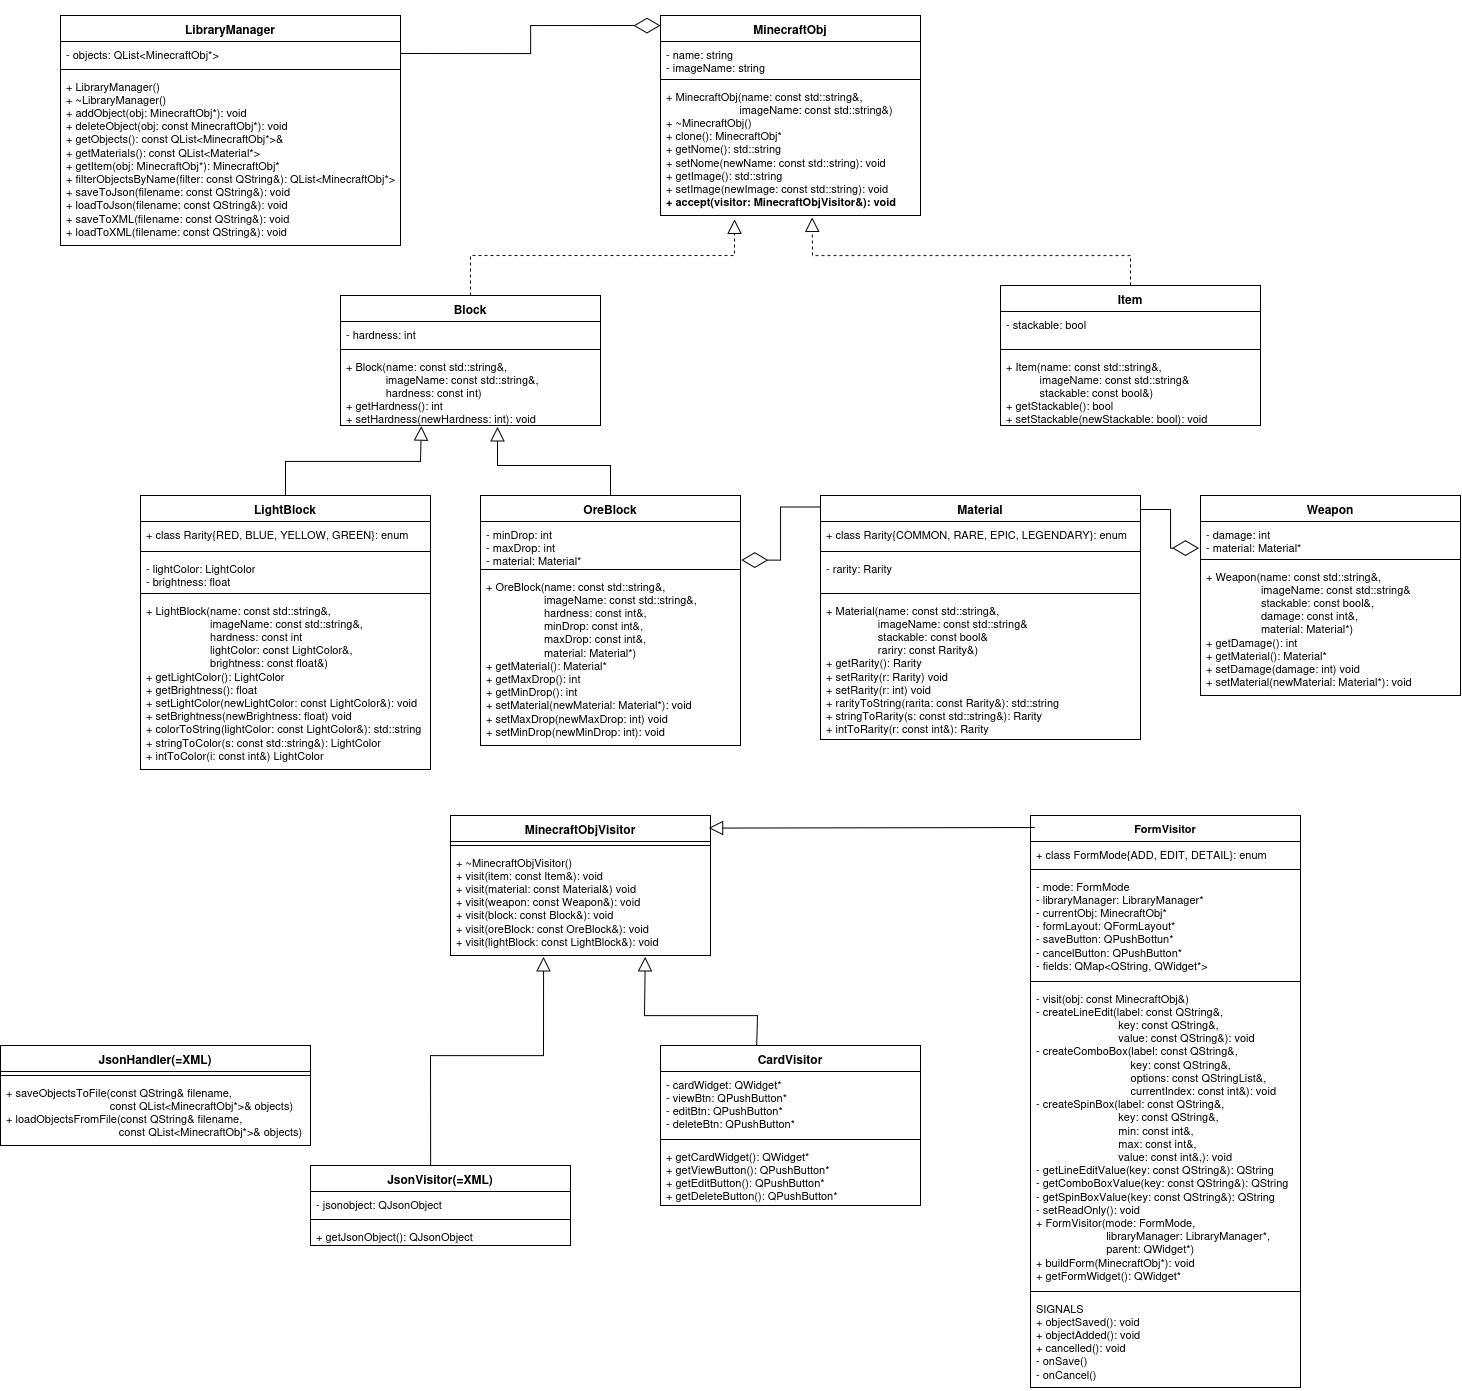
\includegraphics[width=\textwidth]{res/uml-lattico.png}
    \caption{Diagramma UML del modello logico del progetto}
    \label{fig:uml}
\end{figure}

\subsection{Interfaccia Grafica}

La parte di interfaccia grafica (UI) ha il compito di esporre all’utente finale la logica applicativa e le funzionalità implementate, offrendo un’interazione più intuitiva rispetto a un’interfaccia da terminale.  
Tutte le funzionalità di gestione degli oggetti, la visualizzazione e le operazioni sulle liste sono accessibili tramite GUI, costruita con il framework \texttt{Qt}.

Oltre alla classica \texttt{MainWindow}, che gestisce la finestra principale e i menu dell'applicazione, le due componenti più rilevanti dell’interfaccia sono: \texttt{ListView} e \texttt{FormVisitor}.

\texttt{ListView} si occupa di mostrare la lista degli oggetti presenti nel sistema.  
Per rappresentare visivamente ogni oggetto viene utilizzata la classe \texttt{CardVisitor}, che costruisce delle “card” grafiche in grado di sintetizzare visivamente le informazioni salienti di ogni entità, con uno stile semplice ed ergonomico.

\texttt{FormVisitor}, invece, è una componente più complessa: gestisce in un’unica classe le tre operazioni fondamentali che si possono eseguire su un oggetto (escludendo l'eliminazione), ovvero la visualizzazione, la modifica e la creazione.  
L’idea alla base è che queste operazioni condividono la necessità di mostrare e gestire gli stessi attributi, rendendo quindi efficiente centralizzarle in una sola classe, anche a costo di una grafica leggermente semplificata.

Come suggerisce il nome, \texttt{FormVisitor} utilizza il \textbf{design pattern Visitor} per accedere e gestire gli attributi degli oggetti.  
È inoltre supportata da un’enumerazione che specifica in quale modalità operativa il form viene utilizzato (es. \texttt{View}, \texttt{Edit}, \texttt{Create}).

Per motivi di praticità, l’implementazione di \texttt{FormVisitor} si discosta leggermente dall’approccio classico del pattern Visitor, poiché accetta anche un riferimento al \texttt{LibraryManager}.  
Questo permette di gestire direttamente l’inserimento o l’aggiornamento degli oggetti, ad esempio al momento del salvataggio. Si è quindi optato per una soluzione più diretta e funzionale.

\section{Polimorfismo}
\label{sec:polimorfismo}

Come già accennato nelle sezioni precedenti, il polimorfismo è un concetto fondamentale alla base di diversi componenti del progetto.  
Oltre ai classici utilizzi nel modello logico (come nel caso della gerarchia tra \texttt{MinecraftObj}, \texttt{Block} e \texttt{Item}), la sua applicazione più interessante e strutturata è all'interno del \textbf{pattern Visitor}.

La classe base \texttt{MinecraftObjVisitor} definisce i metodi virtuali per visitare ciascun tipo concreto di oggetto. Questi metodi vengono poi sovrascritti all'interno delle classi derivate, che implementano comportamenti specifici a seconda del contesto di utilizzo.  
Il pattern consente quindi di separare la logica operativa dalla struttura dati, rendendo più modulare ed estendibile l’intero sistema.

La prima applicazione concreta di questo pattern è stata nella gestione della \textbf{persistenza dei dati}, con il supporto ai formati \texttt{JSON} e \texttt{XML}.  
Per prendere familiarità con il Visitor, sono stati implementati due \texttt{Handler} specifici per ciascun formato, ciascuno con due funzioni principali: una per la lettura e una per la scrittura dei dati su file.  
Nel caso della scrittura, grazie all’uso di \texttt{JsonVisitor} (e rispettivamente \texttt{XmlVisitor}), ogni oggetto viene trasformato in un \texttt{QJsonObject} (o struttura equivalente per XML), e infine salvato nel file desiderato.

\begin{lstlisting}
    void JsonVisitor::visit(const Block& block) {
    QJsonObject tempJsonObject;
    tempJsonObject["type"] = "Block";
    tempJsonObject["name"] = QString::fromStdString(block.getNome());
    tempJsonObject["imageName"] = QString::fromStdString(block.getImage());
    tempJsonObject["hardness"] = block.getHardness();
    
    jsonobject = tempJsonObject;
    }
\end{lstlisting}

Successivamente, lo stesso approccio è stato esteso anche all'interfaccia grafica.  
La classe \texttt{CardVisitor} sfrutta il pattern Visitor per determinare dinamicamente il tipo dell’oggetto e visualizzarne una rappresentazione sintetica, ad esempio indicando se si tratta di un \texttt{Block}, un \texttt{Weapon} o un \texttt{OreBlock}.  
Tuttavia, la sua implementazione è parziale, poiché mostra solo alcune informazioni specifiche (come il tipo) e non l'intera struttura dell’oggetto.

Una seconda applicazione più completa è rappresentata dalla classe \texttt{FormVisitor}, discussa nella sezione precedente, che usa il Visitor per generare dinamicamente i form di creazione, modifica o visualizzazione, in base alla classe concreta dell’oggetto.  
Questa strategia consente di gestire uniformemente tutti i tipi derivati di \texttt{MinecraftObj} con un'unica struttura logica, evitando lunghe sequenze di \texttt{if} o \texttt{switch}.

\begin{lstlisting}
    void FormVisitor::visit(const Block &block) {
    visit(static_cast<const MinecraftObj&>(block));
    createSpinBox("Durezza:", "hardness", 0, 100, block.getHardness());
    }
\end{lstlisting}

In sintesi, l’uso del polimorfismo tramite il pattern Visitor ha permesso una maggiore flessibilità e modularità sia nella gestione dei dati che nella loro rappresentazione grafica.

\section{Resoconto Ore}
La \textbf{Tabella \ref{tab:rendicontazione}} mostra una stima approssimativa delle ore impiegate nelle varie fasi dello sviluppo del progetto, suddivise per tipologia di attività e tra i due componenti del gruppo.

La ripartizione è stata definita in modo indicativo, dato che il tempo non è sempre stato misurato con precisione e alcune attività sono state svolte in modo informale o durante conversazioni su altri aspetti del progetto. Ciononostante, riflette con buona approssimazione il carico di lavoro e il contributo di ciascuno.

Come si può notare, la parte relativa allo sviluppo dell’interfaccia grafica ha richiesto il maggior impegno. Questo è dovuto in parte al fatto che era una delle prime esperienze con lo sviluppo di GUI: per il sottoscritto rappresentava una sfida nuova, mentre per il mio compagno era un primo approccio assoluto. Inoltre, si è cercato di curare l’aspetto estetico con uno stile semplice e minimalista, il che ha inevitabilmente allungato i tempi.

Infine, le ore dedicate alla stesura della relazione sono divise in funzione delle due relazioni distinte che ciascuno dei componenti del gruppo ha preparato individualmente.

\begin{table}[H]
\centering
\begin{tabular}{|l|c|c|c|}
\hline
\textbf{Attività} & \textbf{Ore Totali} & \textbf{Studente A} & \textbf{Studente B} \\
\hline
Studio e progettazione            & 10 & 6 & 4 \\
Sviluppo del codice del modello   & 20 & 13 & 7 \\
Studio del framework Qt           & 8  & 5 & 3 \\
Sviluppo del codice della GUI     & 35 & 14 & 21 \\
Test e debug                      & 15 & 9 & 6 \\
Stesura della relazione           & 11 & 6 & 5 \\
\hline
\textbf{Totale}                   & \textbf{99} & \textbf{53} & \textbf{46} \\
\hline
\end{tabular}
\caption{Rendicontazione delle ore suddivisa tra i due membri del gruppo}
\label{tab:rendicontazione}
\end{table}

\section{Idee Future}

In una visione a lungo termine, questo progetto potrebbe essere arricchito con ulteriori funzionalità, così da avvicinarsi sempre più a un prodotto completo e realmente utile per lo sviluppo di mod di Minecraft.

Una prima estensione potrebbe consistere nella possibilità, per l'utente, di definire nuove classi personalizzate che rappresentino oggetti specifici del gioco o della propria mod. Tali classi potrebbero essere salvate e caricate in maniera modulare, seguendo una logica simile a quella già adottata per i file \texttt{JSON} e \texttt{XML}, permettendo così una maggiore flessibilità e scalabilità del software.

Un’ulteriore funzionalità utile sarebbe la generazione automatica di file necessari allo sviluppo delle mod, come ad esempio il file \texttt{en\_us.json}, utilizzato per la localizzazione degli identificativi interni degli oggetti nel nome leggibile in inglese.

Queste due evoluzioni andrebbero a rendere il software non solo più completo, ma anche in grado di adattarsi e crescere insieme alle modifiche e agli aggiornamenti del gioco stesso.

\end{document}
